\documentclass{beamer}
\usepackage{inconsolata}
\usepackage{caption}
\usepackage{color}
\usepackage{listings}
\usepackage{subfig}
\usepackage{cooltooltips}
\usepackage{hyperref}
\usepackage{perpage}
\usepackage{graphics}
\usepackage{grffile}
\usepackage{kotex}
\usepackage[normalem]{ulem}
\setbeamertemplate{navigation symbols}{}%remove navigation symbols
\usepackage{listings}
\usepackage{color}
\usepackage{framed}

\definecolor{background}{RGB}{39, 40, 34}
\definecolor{string}{RGB}{230, 219, 116}
\definecolor{comment}{RGB}{117, 113, 94}
\definecolor{normal}{RGB}{248, 248, 242}
\definecolor{identifier}{RGB}{166, 226, 46}



\lstset{
  language=C,               			% choose the language of the code
  alsolanguage=Python,            			% choose the language of the code
  alsolanguage=Java,            			% choose the language of the code
  numbers=none,                   		% where to put the line-numbers
  stepnumber=1,                   		% the step between two line-numbers.        
  numbersep=5pt,                  		% how far the line-numbers are from the code
  extendedchars=true,
  numberstyle=\tiny\color{black}\ttfamily,
  backgroundcolor=\color{background},  		% choose the background color. You must add \usepackage{color}
  showspaces=false,               		% show spaces adding particular underscores
  showstringspaces=false,         		% underline spaces within strings
  showtabs=false,                 		% show tabs within strings adding particular underscores
  frame=single,
  framerule=0pt,
  tabsize=4,                      		% sets default tabsize to 2 spaces
  captionpos=n,                   		% sets the caption-position to bottom
  breaklines=true,                		% sets automatic line breaking
  breakatwhitespace=true,         		% sets if automatic breaks should only happen at whitespace
  title=\lstname,                 		% show the filename of files included with \lstinputlisting;
  basicstyle=\color{normal}\tiny\ttfamily,					% sets font style for the code
  keywordstyle=\color{magenta}\tiny\ttfamily,	% sets color for keywords
  stringstyle=\color{string}\tiny\ttfamily,		% sets color for strings
  commentstyle=\color{comment}\tiny\ttfamily,	% sets color for comments
  emph={True, False, format_string, eff_ana_bf, permute, eff_ana_btr, KeyError,
  ValueError, ZeroDivisionError},
  emphstyle=\color{identifier}\tiny\ttfamily,
  morekeywords={with, as}
}

\lstset{literate=%
   *{0}{{{\color{cyan}0}}}1
    {1}{{{\color{cyan}1}}}1
    {2}{{{\color{cyan}2}}}1
    {3}{{{\color{cyan}3}}}1
    {4}{{{\color{cyan}4}}}1
    {5}{{{\color{cyan}5}}}1
    {6}{{{\color{cyan}6}}}1
    {7}{{{\color{cyan}7}}}1
    {8}{{{\color{cyan}8}}}1
    {9}{{{\color{cyan}9}}}1
}



\newenvironment{enum}{
\begin{enumerate}
  \setlength{\itemsep}{1pt}
  \setlength{\parskip}{0pt}
  \setlength{\parsep}{0pt}
}{\end{enumerate}}

\hypersetup{
  colorlinks=true,
  urlcolor=pink,
}

\MakePerPage{footnote}

\title{파이썬 101}
\subtitle{무한한 라이브러리, 저 너머로!}

\begin{document}
\frame{\titlepage}

\begin{frame}
\frametitle{51일 전: 왜 파이썬?}
\begin{figure}[H]
  \centering
  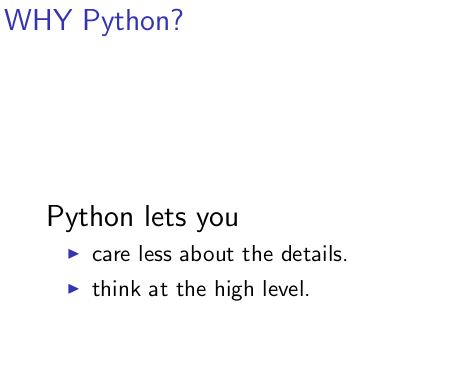
\includegraphics[width=80mm,height=60mm]{recap.png}
\end{figure}
공감 되시나요?
\end{frame}

\begin{frame}
  \frametitle{오늘: 왜 파이썬?}
\begin{figure}[H]
  \centering
  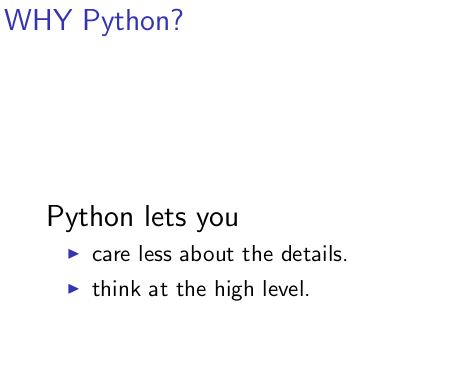
\includegraphics[width=80mm,height=60mm]{recap.png}
\end{figure}
  그리고 다양한 라이브러리들
\end{frame}

\begin{frame}
\frametitle{파이선이 슈퍼히어로라면\ldots}
\begin{figure}[H]
  \centering
  
\includegraphics[width=80mm,height=50mm]{hero.png}
\end{figure}
\end{frame}

\begin{frame}[fragile]
\frametitle{근데 진짜임}
\begin{lstlisting}
import antigravity
\end{lstlisting}
\end{frame}

\begin{frame}
\frametitle{유용한 모듈, 라이브러리와 프로그램들 일부}
\begin{itemize}
\item pdb: 디버깅\\
\item PyPy: 빠른 파이선\\
\item pip: 파이선 패키지 관리자\\
\item Numpy: 빠른 계산\\
\item Pillow: 이미지 처리\\
\item OpenCV: 컴퓨터 비전\\
\item Request: HTTP 요청 주고받기\\
\item Scrapy: 웹크롤링\\
\item Selenium: 웹브라우저 자동화\\
\item KoNLPY: 한국어 처리\\
\item tossi: 한국어 조사처리\\
\item Ren'Py: 비주얼 노벨 \footnotesize\sout{미연시} \normalsize만들기\\
\item Pygame: 2D 게임 만들기\\
\end{itemize}
\end{frame}

\begin{frame}{pdb}
  The Python Debugger
\end{frame}

\begin{frame}[fragile]{지금까지의 디버깅}
\begin{lstlisting}
def wrong_function(n):
    if n == 2 and n == 3:
      print("n is: ", n)
      return True
    if n % 2 == 0 or n < 2:
      print("n is now: ", n)
      return False
    for i in range(3,int(n**0.5+1),2):
        print(n, i)
        if n % i == 0:
            return False
        print("should not print if n is prime", i)
    if n == 3:
      print("if I can read this, I am XXXXed")
    return True
\end{lstlisting}
\end{frame}

\begin{frame}[fragile]{좋은 디버깅}
\begin{figure}[H]
  \centering
  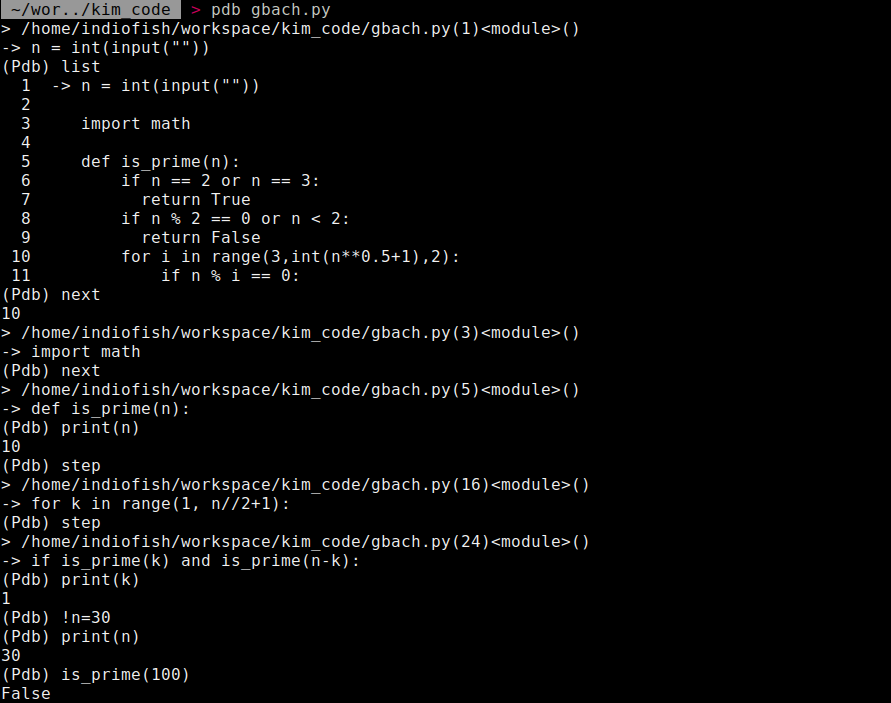
\includegraphics[width=100mm,height=75mm]{pdb_usage.png}
\end{figure}
\end{frame}

\begin{frame}{좋은 디버깅}
\begin{itemize}
  \item help\\
    가능한 명령어를 보여준다.
  \item break (줄번호$\vert$함수이름)\\
    n번째 줄이나 함수에 도달하면 일시정지
  \item print()\\
    우리가 아는 출력함수
  \item !x = 3\\
    값 바꾸기
  \item next\\
    현재 함수의 다음줄로 넘어간다.(중간의 함수는 그냥 실행)
  \item step\\
    step into: 함수 안으로 들어간다.
\end{itemize}
\end{frame}

\begin{frame}{좋은 디버깅}
장점들
\begin{itemize}
  \item 프로그램을 껐다켰다하지 않고도 테스트 가능
  \item 프로그램을 바꾸지 않고도 테스트 가능
  \item 멋있음
\end{itemize}
\end{frame}

\begin{frame}{PyPy}
\begin{figure}[H]
  \centering
  
\includegraphics[width=80mm,height=20mm]{pypy-logo.png}
\end{figure}
  Python으로 실행하는 Python
\end{frame}

\begin{frame}{PyPy}
  python program.py == pypy program.py\\
  JIT 컴파일과 파이선 코드를 C로 번역하는 과정 등을 거쳐 표준 python 구현체보다
  2-10배 정도 빠를 때도 있고, 조금 느릴 때도 있습니다.
\end{frame}

\begin{frame}{pip}
\textit{pip install you-name-it}\\
  파이썬에 기본적으로 포함되어 있는, 패키지 관리자. 일일이 홈페이지에 들어가서
  설치파일을 받지 않아도 되는 장점이 있습니다.
\end{frame}

\begin{frame}{Numpy}
\textit{pip install numpy}\\
Anaconda 등에 포함되어 있어 써보셨을 것 같은 Numpy\\
\end{frame}

\begin{frame}{왜 Numpy?}
  딥러닝 등의 근간이 되는 행렬\footnote{김모 교수님 \textit{"미적분학은 한물갔고 이젠 선형대수학의
  시대입니다 음하하!"}}을 빠르게 계산 해줍니다.
물론 그외에도 많은 수학기능이 있습니다.
\end{frame}

\begin{frame}[fragile]{Numpy}
\begin{lstlisting}
import numpy as np
SIZE = 500
a = np.array([[randint(-100,100) for _ in range(SIZE)] for _ in range(SIZE)])
b = np.array([[randint(-100,100) for _ in range(SIZE)] for _ in range(SIZE)])
c = np.dot(a, b)
\end{lstlisting}
500 x 500 행렬의 곱셈
\end{frame}

\begin{frame}[fragile]{Numpy vs 저}
\begin{figure}[H]
  \centering
  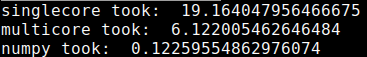
\includegraphics[width=75mm,height=20mm]{./numpy-result.png}
\end{figure}
코드는 깃 저장소의 mat\_mul.py에서 확인 가능합니다.
\end{frame}


\begin{frame}{Pillow}
\textit{pip install Pillow}\\
Python Image Library (PIL)의 변형판\\
사진을 늘리고, 줄이고, 변형하는데 유용합니다.\\
https://pillow.readthedocs.io/en/stable/
\end{frame}

\begin{frame}{Pillow}
\begin{lstinputlisting}
  {pil_test.py}
\end{lstinputlisting}
\end{frame}

\begin{frame}{OpenCV}
\textit{pip install opencv-python}\\
https://docs.opencv.org/master/d6/d00/tutorial\_py\_root.html\\
이미지처리 + 컴퓨터비전을 위한 라이브러리.\\
Pillow보다 강력하지만, 복잡하네요\\
컴퓨터비전 이론을 몰라도 Ctrl CV로 사용할 수 있으나, 왜 결과가 나오는 지 모를 수가 있음.
\end{frame}

\begin{frame}{심슨}
\begin{figure}[H]
  \centering
  
\includegraphics[width=100mm,height=60mm]{simpsons.jpeg}
\end{figure}
\end{frame}

\begin{frame}{누구 눈일까요? 5초}
\begin{figure}[H]
  \centering
  
\includegraphics[width=20mm,height=20mm]{eyes3.jpeg}
\end{figure}
\end{frame}

\begin{frame}{OpenCV - Template Matching Ctrl CVed}
\begin{lstinputlisting}
  {cv_test.py}
\end{lstinputlisting}
\end{frame}

\begin{frame}{아하.}
\begin{figure}[H]
  \centering
  
\includegraphics[width=100mm,height=60mm]{res.png}
\end{figure}
\end{frame}

\begin{frame}{Requests}
\begin{lstinputlisting}
  {cv_test.py}
\end{lstinputlisting}
\end{frame}

\begin{frame}{Requests}
\textit{pip install requests}\\
HTTP 요청\footnote{비약하면 인터넷에서 보는 것}을 주고받는 모듈\\
https://2.python-requests.org/en/master/
\end{frame}

\begin{frame}{Requests}
\begin{lstinputlisting}
  {namu_read.py}
\end{lstinputlisting}
나무위키 링크에서 무언가 받아오기
\end{frame}

\begin{frame}{Requests}
\begin{lstinputlisting}
  {insta_login.py}
\end{lstinputlisting}
인스타그램 로그인 하기
\end{frame}

\begin{frame}{Requests - 단점}
사이트마다 이런 종류의 접속을 막기 위해 다양한 방법을 사용해서,
사이트의 구조를 잘 찾아봐야 짤 수 있고, 귀찮다.

정적인 웹페이지에서는 잘 되지만, js를 많이 사용하는 동적인 웹페이지는 정보를
  받아오기 어렵다.
\end{frame}

\begin{frame}{그래서 Selenium}
\textit{pip install selenium}\\
브라우저를 직접 이용하여, 웹사이트에 접근 할 수 있다.\\
만든 웹앱을 테스트하는 용도의 프로그램이지만, 얼마든지 응용 가능.
\end{frame}

\begin{frame}{Selenium}
\textit{pip install selenium}\\
+\\
자기가 사용할 브라우저의 웹드라이버를 설치해야 한다.\\
크롬: https://sites.google.com/a/chromium.org/chromedriver/downloads\\
파이어폭스: https://github.com/mozilla/geckodriver\\
익스플로러: ??

화면뜨는 것이 싫다면, headless 크롬을 이용하면 된다.
\end{frame}

\begin{frame}{Selenium}
\begin{lstinputlisting}
  {snulogin.py}
\end{lstinputlisting}
\end{frame}

\begin{frame}{Selenium}
\begin{lstinputlisting}
  {instalogin.py}
\end{lstinputlisting}
\end{frame}

\begin{frame}{Selenium}
특정 HTML 요소에 접근하는 다양한 방법이 있고, 되는 방법도, 안되는 방법도
  있습니다 (복불복?)
\end{frame}

\begin{frame}{Selenium}
인터넷에서 이것저것 긁어왔는데, 그 다음엔?
\end{frame}

\begin{frame}{KoNLPy}
한국어 처리 라이브러리
\end{frame}

\begin{frame}{KoNLPy}
설치하기가 조금 까다로워서 불편합니다.\\
https://konlpy-ko.readthedocs.io/ko/v0.4.3/\#start
\end{frame}

\begin{frame}{KoNLPy}
\begin{figure}[H]
  \centering
  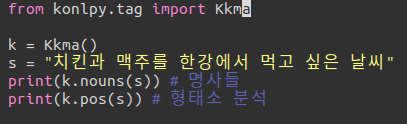
\includegraphics[width=90mm,height=30mm]{korean.png}
\end{figure}
\end{frame}

\begin{frame}{Tossi}
\begin{figure}[H]
  \centering
  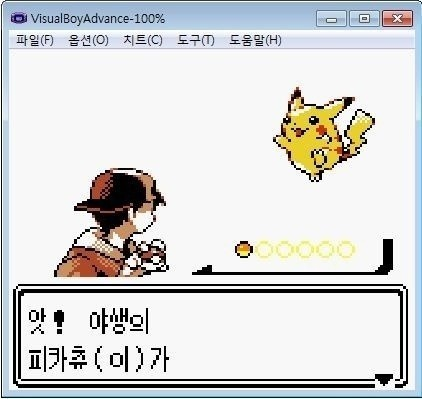
\includegraphics[width=50mm,height=50mm]{poke.jpg}
\end{figure}
이런 문제(을)를 해결하는 라이브러리입니다.\\
https://github.com/what-studio/tossi
\end{frame}

\begin{frame}{게임제작툴}
은 생략.
\end{frame}

\begin{frame}{다른 라이브러리들?}
\begin{figure}[H]
  \centering
  
\includegraphics[width=80mm,height=50mm]{google.png}
\end{figure}
\end{frame}

\end{document}
